\documentclass[aps,pre,12pt,preprint,%
	onecolumn,showpacs,showkeys,nofootinbib]{revtex4-2}
%Chinese
	\usepackage[UTF8,fontset=fandol]{ctex}
%	\usepackage[datesep=/]{datetime2} % Use default
	\DeclareTextFontCommand{\textbf}{\sffamily}
%Presenting
	\usepackage[table]{xcolor}
	\usepackage{graphicx}
	\usepackage[font=small,format=plain,%
		labelfont=bf,textfont=it,%
		singlelinecheck=false]{caption}
	\usepackage[above]{placeins}
%	\usepackage{float} % Cause trouble for table footnotes
	\usepackage{wrapfig}
	\usepackage{tabularx,array,booktabs,multirow,bigstrut}
	\newcolumntype{C}[1]{>{\hsize=#1\hsize%
		\centering\arraybackslash}X}
	\newcommand{\minitab}[2][l]{%
		\begin{tabular}{#1}#2\end{tabular}}
	\usepackage{setspace,dcolumn}
	\usepackage{subfig}
	\usepackage{psfrag,epsfig}
%MathSetting
	\let\latexointop\ointop
	\usepackage{amsmath,bm,amssymb,esint,extarrows}
	\usepackage{upgreek,textcomp,mathrsfs}
	\usepackage[only,sslash]{stmaryrd}
	\usepackage{nicefrac,eqnarray}
%	\usepackage{amsthm} % Enable when necessary
%	\usepackage[mathscr]{eucal} % Enable when necessary
	\usepackage{mathtools,physics,siunitx}
	\usepackage{stackengine,varwidth}
	\usepackage{tikz}
	\usepackage{resizegather,empheq}
	\usetagform{default}
	\usepackage{calligra,fourier-orns}
	% Keep \oint unchanged by esint
	\let\ointop\undefined
	\let\ointop\latexointop
	% Define a scriptr 
	\DeclareMathAlphabet{\mathcalligra}{T1}{calligra}{m}{n}
	\DeclareFontShape{T1}{calligra}{m}{n}{<->s*[2.2]callig15}{}
	\newcommand{\scriptr}{\mathcalligra{r}\,}
	\newcommand{\rvector}{\pmb{\mathcalligra{r}}\,}
	% Useful shorthand
	\DeclarePairedDelimiter\ave{\langle}{\rangle}
	\newcommand\inlineeqno{\stepcounter{equation}\ (\theequation)}
	\newcommand{\sinc}{\operatorname{sinc}}
	\newcommand{\mbb}[1]{\mathbb{#1}}
	\newcommand{\mrm}[1]{\mathrm{#1}}
	\newcommand{\mcal}[1]{\mathcal{#1}}
	% Scaling and positioning
	\newcommand\scalemath[2]{\scalebox{#1}{\mbox{\ensuremath{\displaystyle #2}}}}
	\newcommand\raisemath[2]{\raisebox{#1\depth}{${#2}$}}
	\empheqset{box=\nicebox}
	% Presenting
	\newcommand*\nicebox[1]{\fbox{\hspace{1em}\addstackgap[5pt]{#1}\hspace{1em}}}

	\allowdisplaybreaks[2]
%ParagraphSetting
	\setlength{\parskip}{.3\baselineskip}
	\usepackage[defaultlines=2,all]{nowidow}
	\postdisplaypenalty=50
%PageSetting
	\usepackage{titlesec}
	\titleformat*{\section}{\large\bfseries}
	\usepackage[colorlinks=true,linkcolor=blue]{hyperref}
	\newcommand{\texstringonly}[1]{%
		\texorpdfstring{#1}{}}
	\usepackage[vmargin={3.5cm,4cm},hmargin=3cm,%
		footnotesep=\baselineskip]{geometry}
%	\usepackage[bottom]{footmisc} % Cause trouble for table footnotes
	\usepackage{changepage}
	% Autoref names
	\renewcommand{\tableautorefname}{\tablename}
	\renewcommand{\figureautorefname}{\figurename}
	% List settings
	\usepackage{enumitem}
	\setlist{itemsep=0pt,topsep=0pt,labelindent=\parindent,leftmargin=0pt,itemindent=*}
	% Some redefined lengths
	\setlength{\headsep}{1.6\baselineskip}
%	\setlength{\footnotesep}{3\parskip} % Use when necessary
	% Header
	\usepackage{fancyhdr,lastpage}
	\pagestyle{fancy}
%	\fancyhf{} % Clear default settings; disabled for now
	\cfoot{--\ \thepage\,/\,\pageref{LastPage} \ --}
	\setlength{\footskip}{2\baselineskip}
	\renewcommand{\headrulewidth}{0.1pt}
	\renewcommand{\headrule}{
		\ifnum\value{page}=1\relax\else
			\vbox to 2pt{
			\hbox to \headwidth{\dotfill}\vss}
		\fi}
	\fancypagestyle{titlepagestyle}{%
		\fancyhead{}
		\chead{
			\vspace{2.5\baselineskip}
			
\includegraphics[width=.75\linewidth]{../PKUPhy}}
	}
	% Separator
	\newcommand{\newparagraph}{\pagebreak[3]\noindent%
		\hfil
		~\raisebox{-4pt}[10pt][10pt]{\decofourright~~~~~~~~\decofourleft}~ %
		\par
	}
%	% Background % Use when necessary
%	\usepackage{background} %Waterstamp package
%	\SetBgContents{...的实验报告} %Waterstamp to prevent copying
%	\SetBgScale{5} %Waterstamp setting
	% Essay format
	\renewcommand\appendixname{附录}
	\renewcommand\abstractname{}
	\renewcommand\tablename{表}
	\renewcommand\figurename{图}
	\renewcommand\refname{参考文献}
	\renewcommand\contentsname{目录}
	\makeatletter
	\def\@pacs@name{\songti\zihao{-4}{\bf PACS码:}}
	\def\@keys@name{\songti\zihao{-4}{\bf 关键词:}}
	\def\Dated@name{日期:}
	\def\Received@name{\zihao{-5}{接收} }
	\def\Revised@name{\zihao{-5}{修订} }
	\def\Accepted@name{\zihao{-5}{采纳} }
	\def\Published@name{\zihao{-5}{发表} }
	\makeatother
	\linespread{1.5}
	\renewcommand{\labelenumi}{\alph{enumi}.}
	\leftmargini=20mm
	\newcommand{\supercite}[1]{\textsuperscript{\,%
		[\citenum{#1}]}}
	\let\fancycite\cite
	\renewcommand{\cite}[1]{\textup{\fancycite{#1}}}

%Miscellaneous
%	\newcommand{\tabindent}{\hspace{2em}}
%FourierTransform
	\newcommand{\fourierf}{\mathscr F}
\begin{document}
%Basic Data
	\title{%
	\texstringonly{\hfil\\[2\baselineskip]}
	\sf\LARGE%
		非线性晶体中的二倍频与和频%
	\texstringonly{\vspace{3ex}}}
	\author{\fangsong\large%
		吴熙楠%
	\vspace{2mm}}
	\affiliation{\it%
		北京大学物理学院~~学号:\normalfont 1900011413\,}
	\date{\today}
	\keywords{二倍频与和频; KDP 晶体; 相位匹配条件}
	\email{xinanwu@pku.edu.cn;}
	
\begin{abstract}
\vspace{10mm}
\begin{spacing}{1.5}\normalsize
\setlength{\parskip}{.3\baselineskip}
%	200—300字,
%	说明用什么方法做了什么事,
%	由此得到什么结果和结论,
%	有何意义. 
%	不用缩略词,不用第一人称.
%	
本实验中利用 1.06$\mu m$ 的 YAG 固体激光器和 KDP 倍频晶体对倍频现象进行了观察, 定量分析了相位匹配条件附近光强随着晶体角度的变化, 加深了对于相位匹配条件的认识. 实验中还对倍频的激光的波长进行了鉴定, 得到的波长确实为 0.53$\mu m$, 从而证实了得到绿色激光为倍频光.
\end{spacing}
\end{abstract}
\clearpage
\maketitle
\thispagestyle{titlepagestyle}
%
%	\item 课程实验报告应假定读者既不是已知全部实验细节的指导教师,也不是缺少专业知识的公众,而是同领域的实验研究者,或审稿人. 不能要求读者要在读过课程讲义后才能读懂课程实验报告.
%	\item 公式、图和表要分别用阿拉伯数字编列序号. 公式和图表要达到可发表的质量.
%	\item 凡不是自己独立思考得到的内容都应该引参考文献. 不能大段引用同一参考文献. 对复杂问题,应该优先考虑引用参考文献得到结果. 对简单一些的问题才鼓励独立思考.
%	\item 较长的推导和说明可以作为附件提交,不占用报告篇幅.
%	\item 思考题不是报告的组成部分. 应另起一页附在报告的最后.

\newpage
\section{引言}
%	研究论文引言一般包含以下内容:
%	(1)所研究领域背景和现状;
%	(2)有待研究的问题;
%	(3)本研究的目的、主要内容和结果;
%	(4)结果的意义.\par
%	在写实验报告的引言时,同学可以假想自己是第一个做类似研究的人.\par
%	引言一定要切合报告正文,不能漫无目的地介绍背景. 要快速地将读者引导到报告主题上,并作较深入的讨论.\par
%	引言篇幅可以在较大范围内变化,但最长不应超过报告文字篇幅的1/3.\par
%	引言撰写可以参考实验讲义,可以复述,但不能复制讲义上的任何一句话.\par
%%%%%%%%%%%%%%%%%%%%%%%%%%%%%%
激光产生以后能产生的光强被极大提升了, 这使得人们对于强光下光与物质相互作用的研究得以实现. 强光与物质相互作用中的一个效应是非线性效应, 即会产生二倍频,三倍频,和频,差频等等效应, 产生了许多的应用. 本实验中便对于倍频现象进行观察以及对相位匹配条件进行定量分析, 从而加深对于非线性效应的理解.
\section{理论}
\subsection{非线性光学基础}
激光与物质的非线性作用,可以写成极化强度矢量的表达式形式:
\begin{equation}
    \label{eq:nonlinear}
    \vec{P} = \chi^{(1)}\vec{E} + \chi^{(2)}\vec{E}\vec{E} +
    \chi^{(3)}\vec{E}\vec{E}\vec{E} + \cdots
\end{equation}
\par 当入射光的电场很小时,表达式\ref{eq:nonlinear}中的非线性项可以忽略,产生的偶极子实际上与电场
正比,这就是线性光学现象。但当入射光的电场较强时,非线性项不能再被忽略,因而可观测到产生的二次倍频、和频以及差频等现象,需要注意的是对于中心对称晶体或者各向同性晶体不会出现二阶非线性效应。但是想要观察到二阶非线性效应还需要满足波矢的相位匹配,如果相位匹配条件不满足,则非线性转换效率会变得很低无法观测到,在本次实验中我们使用的非线性晶体是KTP(磷酸钛氧钾),利用角度调谐的方法调制相位匹配。
\subsection{相位匹配方法}
极化强度与入射光强和非线性极化系数有关, 但与此同时, 相位匹配也对出射光强起着很大的作用.
	\begin{figure}[!h]
	\centering
	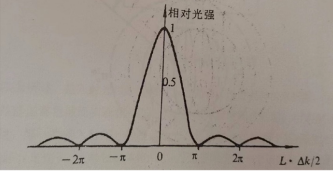
\includegraphics[width=.9\linewidth]{img/1.png}
	\caption[倍频效率与$\Delta kL/2 $的关系]{倍频效率与$\Delta kL/2 $的关系}\vspace{1ex}
	\end{figure}
    \par 倍频转化效率推导可得:$\eta\propto \dfrac{sin^2(\Delta kL/2)}{(\Delta kL/2)^2}$,因而要获得最大的转换效率, 就要使$\Delta kL/2=0$. 由于 L>0, 因而要使得$\Delta k=0$, 即$n^\omega=n^{2\omega}$, 即基频光与倍频光折射率相等的时候倍频光较强, 这杯称为相位匹配条件. 从物理上理解, 相位匹配条件就是让基频光在晶体中沿途个点激发的倍频光传播到出射面的时候具有同样的相位.
    \par 实现相位匹配条件的方法: 介质中一般存在正常色散效应, $n^{2\omega}-n^\omega$
    大约为$10^{-2}$量级. 而在各向异性介质中, 由于存在双折射, 可以利用不同
    偏振光之间的折射率关系, 实现相位匹配条件. 比如在负单轴晶体中, 折
    射率球面如图 2 所示, 在实线与虚线相交的地方即为基频光与倍频光折射
    率相等的地方. 所以光沿着与光轴成$\theta_m$角度传播的时候, 基频光中 o 光的
    折射率可以和倍频光中 e 光的折射率相等, 从而实现相位匹配条件. $\theta_m$就
    称为相位匹配角. 在实验中往往就把晶体按特定方向切割, 使得晶面法向
    与光轴夹角即为相位匹配角.
    	\begin{figure}[!h]
    	\centering
    	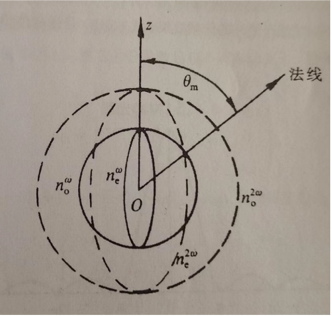
\includegraphics[width=.7\linewidth]{img/2.png}
    	\caption[负单轴晶体折射率球面示意图]{负单轴晶体折射率球面示意图}\vspace{1ex}
        \end{figure}
        \par 相位匹配条件有两类. 第一类是入射同一种线偏振光, 然后负单轴晶
        体将两个基频 o 光光子转换成一个倍频的 e 光光子, 正单轴晶体将两个基
        频 e 光光子转换成一个倍频的 o 光光子. 第二类是将一个基频 e 光光子与
        一个基频 o 光光子转换为一个 e 光或者 o 光光子.
\section{实验装置}
%	在此部分需要将实验条件交待清楚到别人能重复你的实验结果的程度. 此外,还需表明你已尽了最大努力来提高实验精度和结果的可靠性. 简单的不确定度估计可以在此节给出,复杂一些的可以放到分析讨论部分.\par
%	实验条件不仅是指直接影响实验结果的实验参量,而且还包括影响实验质量和可靠性的因素,如室温、空气湿度、基真空、原材料纯度等.\par
%	作为教学实验报告,此节写详细一点没有坏处.\par
%	成段有叙述,必要才分节。
%%%%%%%%%%%%%%%%%%%%%%%%%%%%%%
\begin{figure}[!h]
    	\centering
    	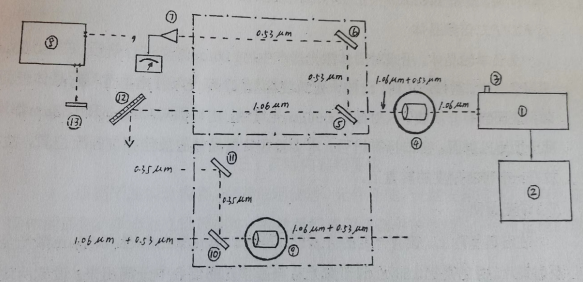
\includegraphics[width=1.0\linewidth]{img/3.png}
    	\caption[实验装置示意图]{实验装置示意图}\vspace{1ex}
        \end{figure}
        \par 实验示意图如上图所示. 1 为 YAG 固体激光器, 产生 1060nm 红外激
        光, 其倍频后为 530nm 绿光激光. 2 为电源以及冷却系统. 3 为倍频拉
        杆, 杆推进去的时候会把倍频晶体加入到光路中, 从而产生 530nm 绿光.
        4为KDP 二倍频负单轴晶体, 已经按一定角度切好, 光垂直于入射晶体表
        面的时候基本达到相位匹配条件, 实验中通过改变这块晶体的方向来观察
        相位匹配条件的影响; 晶体两面镀有膜, 入射面对 1.06$\mu m$ 增透, 出射面对
        1.06$\mu m$和 0.53$\mu m$ 均增透. 5 ,6 为反射镜, 对 1.06$\mu m$ 全透, 对 0.53$\mu m$
        全返, 用于分离出 0.53$\mu m$ 激光. 7为功率计. 8为单色仪, 用于对可见和紫
        外光进行波长鉴定. 9为KDP 三倍频负单轴晶体, 对 1.06$\mu m$ 和 0.53$\mu m$ 的
        光进行合频, 产生0.35$\mu m$的紫外光. 10 ,11为反射镜, 对1.06$\mu m$,0.53$\mu m$
        全透, 对 0.35$\mu m$ 全返, 用于分离出0.35$\mu m$ 激光. 12为散射片, 终止激光.
        13为白纸屏, 用于观察绿色激光强弱.
        \par 实验中先测定二倍频实验中相位匹配条件的影响, 然后对倍频激光波长值进行标定.
        \par 光路搭建的时候, 出于方便, 应当在 YAG 激光器倍频拉杆产生 0.53$\mu m$
        可见绿光下进行. 光路搭建好之后, 中间部分就不再随意移动, 搬动拉杆使得激光器换至 1.06$\mu m$ 红外波段.
\section{结果与分析}
%	实验结果应尽量以图表的形式给出. 每一个图表都应该是完整的,即阅读图表时可以不必依赖正文.\par
%	依自己意愿,实验结果和对结果的分析讨论既可分为两节也可合在一节.\par
%	\begin{table}[h]
%	\caption{元件恒流大小,为什么要左对齐呢?奇怪。}
%	\small
%	\begin{tabularx}{.6\linewidth}{C{.3} C{1}}
%	\toprule
%	\midrule
%		元件\footnote{%
%			注释一个看看%
%		} & 恒流大小\footnote{%
%			再开一个!哈哈
%		} \\
%	\midrule
%		Pt  &
%			$\SI{1.00005}{\mA}
%				= \SI{100.005}{\mV} / \SI{100}{\ohm} $ \\
%	\midrule
%	\bottomrule
%	\end{tabularx}
%	\label{tab:ExTab}
%	\end{table}
%	
%	每个图一般包含:图名、轴名、轴、刻度、标尺、数据点、曲线、图例、标注和图注等部分. 应尽量让读者不看正文就能基本理解图的含意.\par
%	逐点测量得到的函数关系要同时用表格和图给出. 需要作比较的多条曲线要画在同一图上.\par
%	为避免读者在图表和正文间反复跳跃阅读,在正文中也要对图表作必要的说明.\par
%	
%	对于预料之外的实验结果,必须首先小心证明其可靠性.读者只有在相信你的实验结果时才愿意花时间看你的分析.\par
%	必须用文字归纳整理出正式的实验结果或结论.可信的实验结果是课程报告最重要的内容.作为一个实验物理工作者,分析解释出错并不丢脸,实验结果不被采信则是致命的.\par
%	教学实验的结论往往是预先知道的. 所以,教师更关心的是你的说理过程. 一般说来,单由课内实验的结果不足以能得到明确的结论. 此时,你可以引用他人的研究结果来帮助帮助自己的论证,但必须注明出处. \par
%	确实不能得到明确结论时,可以给出几种可能结论并指出可以再做哪些实验来帮助作进一步的判断.\par
%	总之,分析讨论部分要做到: 论据要valid,论证要reasonable,结论要convincing.\par
%%%%%%%%%%%%%%%%%%%%%%%%%%%%%%

\section{结论}
%	首先要给出实验结果,然后再给出由实验结果分析得到的结果和结论.此部分给出的内容要比摘要中的全面,用词要更准确.\par
本实验中对相位匹配条件进行了定量测量, 在相位匹配角附近倍频光光强会随着小的角度偏移而大幅下降, 从而对相位匹配进行了验证. 实验中还利用单色仪对倍频后的激光波长进行了测量, 测量值为$\lambda_{2\omega} =(530.48 \pm 0.10)nm$,为 1.06$\mu m$ 激光波长的一半, 从而证实了其为倍频激光.通过本实验, 加深了对于非线性效应的理解以及更加熟悉了搭光路的过程,为以后进行类似的实验做了准备.
\section{思考题}
1.欲获得0.35$\mu m$的紫外激光, 为何采用1.06$\mu m$和0.53$\mu m$和频的方法, 而不是用对1.06$\mu m$光直接三倍频的方法?
\par 答:因为三倍频的倍频效率要比两束光和频的效率要低很多, 因而如果直接三倍频光可能会很弱以至于探测不到.

2.为满足三倍频晶体对输入光的偏振态的要求, 如何判定1.06$\mu m$和0.53$\mu m$两种光的偏振方向? 
\par 答:利用一个偏振片, 对进入合频晶体前和从晶体出射的光偏振情况进行比较; 晶体要调到相位匹配角. 绿光应当只有一个偏振态, 红外光可能两个偏振的光都有.如果红外光只有一个偏振态, 则若偏振片转动至某个角度的时候进入晶体前的光中既看不到绿光也用相纸检测不到红外光, 则两个光的偏振相同; 如果看不到红外光和看不到绿光的情形中偏振片相差90度, 则两个光的偏振态不同.如果红外光两个偏振态都有, 则比较进入晶体前和从晶体出射的光的偏振态. 如果红外光中和绿光相同偏振的光减弱了, 则合频所用的两光的偏振相同; 如果红外光中和绿光不同偏振的光减弱了, 则合频所用的两光的偏振不同.

3.如何知道本实验的倍频为第二类相位匹配?
\par 答:利用一个偏振片, 对进入倍频晶体前和从晶体出射的光偏振情况进行比较; 晶体要调到相位匹配角. 红外光中应该是o光和e光都有, 而出射绿光应该只有一种偏振态. 如果经过晶体后, 红外光中和出射绿光相同偏振以及不同偏振的光都减弱了, 则倍频所用的两光的偏振不同, 为第二类相位匹配; 如果经过晶体后, 红外光中和绿光不同偏振的光明显减弱了, 而和绿光相同偏振的光相对而言没有明显减弱, 则合频所用的两光的偏振相同, 为第一类相位匹配条件.

4.在用纸板接收0.35$\mu m$的紫外激光的时候, 会看到有紫光和弱的绿光, 这紫光是否就是紫外激光? 紫光和绿光各是什么原因产生的? 用单色仪能测量紫光波长吗? 为什么? 
\par 答:紫光应该不是紫外激光, 可能是紫外光激发纸板上分子或灰尘产生的荧光; 绿光可能也有荧光的成分, 也可能是没被完全滤掉的绿色激光. 单色仪可以确定紫光波长, 但可能由于其太弱而使得信号太弱, 探测不到.
\section{致谢}
%	此部分感谢同组人...和对实验和报告有帮助的人.
	感谢我的合作伙伴杨轩同学,他的工作是不可或缺的;感谢耐心的胡小永指导老师对我们的巨大帮助。
\begin{thebibliography}{99}
	\addcontentsline{toc}{section}{参考文献}
	\bibitem{ref1}北京大学物理学院光学所, 激光实验, 第二版, 北京: 北京大学物理学院, 2023.
\end{thebibliography}
\clearpage
\end{document}
